The chosen benchmark problem is the following:
\begin{linenomath}
	%\begin{subequations}
	\begin{align}
		\min_{\bm{x}\in \mathbb{R}^{n}} \quad & \sum_{i = 1}^n x_{i}^2 - \sum_{i = 1}^{n-1} x_{i}x_{i+1} + \sum_{i = 1}^n x_{i} \label{Sec1_Eq_problem} \\
		\text{subject to} \quad & x_{1} + x_{1+K} +  x_{1+2K} +\cdots = 1, \nonumber\\
		& x_{2} + x_{2+K} +  x_{2+2K} +\cdots = 1,  \nonumber\\
		& \quad\quad\quad\quad\quad\quad\vdots \nonumber\\
		& x_{K} + x_{2K} +  x_{3K} +\cdots = 1, \nonumber\\
		& x_{i} \geq 0, \quad i = 1, \dots, n,\nonumber
	\end{align}
	%\end{subequations}
\end{linenomath}
The problem above can be reformulated as in \ref{Sec1_Eq_prb_mat} if we consider the following matrices:

\begin{linenomath}
	%\begin{subequations}
	\begin{align}
		&\mathbf{Q} = 
		    \begin{bmatrix}
		        2 & -1 &  &  & 0 \\
		       -1 & \ddots & \ddots &  &   \\
		         &\ddots &  \ddots & &   \\
		         &  &  &  &    -1 \\
		         0 &  &  &  -1 & 2
		    \end{bmatrix}\in \mathbb{R}^{n\times n}
		    &\bm{c} = \begin{bmatrix}
		        1 \\ 1 \\ \vdots \\ 1
		    \end{bmatrix}\in \mathbb{R}^{n}, \nonumber\\
		    &\mathbf{A} = 
		    \begin{bmatrix}
		    1 &      & &  1  &     &  &  &    1  &     &\\
		    & \ddots & &  & \ddots &  &  \ddots&   & \ddots &\\
		    &   &    1 &  &     &  1  &  &   &  &     1
		    \end{bmatrix}\in \mathbb{R}^{K\times n}
    		&\bm{b} = \begin{bmatrix}
		        1 \\ 1 \\ \vdots \\ 1
		    \end{bmatrix}\in \mathbb{R}^{K}. \nonumber\\
		\end{align} 
	%\end{subequations}
\end{linenomath}

Ultimately, the problem will be solved in the more general formulation \ref{Sec2_Eq_yolo} using $\hat{\mathbf{A}}\in \mathbb{R}^{(2K + n)\times n}$ and $\hat{\bm{b}}\in \mathbb{R}^{2K + n}$ as defined in \ref{Sec2_Eq_A_hat_B_hat}.\\
\\
\noindent We studied four size scenarios, with $n=10^4, n=10^5$ and $K=100, K=500$. We tested both methods for solving the linear system as shown in \ref{ls_sol} using both formulations \ref{sec2_eq_augmented} and \ref{Sec2_Ee_SUS}. Moreover, we compared our implementation of the GMRES algorithm with its native implementation in MATLAB\\
\\
\noindent We initialized $\bm{y}_0 = \texttt{ones(2*K+n,1)}$, $ \hat{\bm{\lambda}}_0 = \texttt{ones(2*K+n,1)}$ and we obtain $\bm{x}_0$ by solving the slack variable constraint in \eqref{Sec1_Eq_kkt_after} in the \textit{least squares} sense. As seen in  \eqref{Sec3_eq_tau} we have chosen the parameter $\tau_k \in [0,1]$ to be a function on $\mu_k$ because we wanted $\tau_k$ to converge to $1$ as $\mu_k$ approaches to 0. After  \textit{tuning} the parameters, we have chosen the following expression:
\begin{equation}
    \tau_k := \tau(\mu_k) = 0.3 \exp{(-\mu_k)} + 0.7.
\end{equation}

In the following table computational times are shown comparing our implementation of the GMRES algorithm with the native implementation in MATLAB.
{\begin{center}
    \begin{tabular}{|l|c|c|c|r|} 
     \hline Dimensions & L.S. Formulation &Time $[s]$ Native & Time $[s]$ Our GMRES \\
       \hline    
       $ n=10^4$, $K=100$ & Aug & $ 0.561$ &$0.439$  \\
       \hline
       $ n=10^4$, $K=100$ & Sus & $ 0.592$ &$0.386$  \\
       \hline
       $ n=10^4$, $K=500$ & Aug & $ 1.191$ &$0.262$  \\
       \hline
       $ n=10^4$, $K=500$ & Sus & $ 2.383$ &$1.407$  \\
       \hline
       $ n=10^5$, $K=100$ & Aug & $ 1.663$ &$2.965$  \\
       \hline
       $ n=10^5$, $K=100$ & Sus & $ 2.383$ &$2.408$  \\
       \hline
       $ n=10^5$, $K=500$ & Aug & $ 1.311$ &$1.229$  \\
       \hline
       $ n=10^5$, $K=500$ & Sus & $ 5.413$ &$5.601$  \\
       \hline

  \end{tabular}
  
\end{center}}

As it is visible in the table above, performing the algorithm using the \ref{sec2_eq_augmented} formulation of the linear systems performs much quicker the majority of times. Let's investigate how the computation times scale with the dimension of the problem, fixing the value \(K=100\) and solving the \ref{sec2_eq_augmented} formulation.

\begin{figure}[H]
    \centering
    \subfloat[1][Native GMRES algorithm]{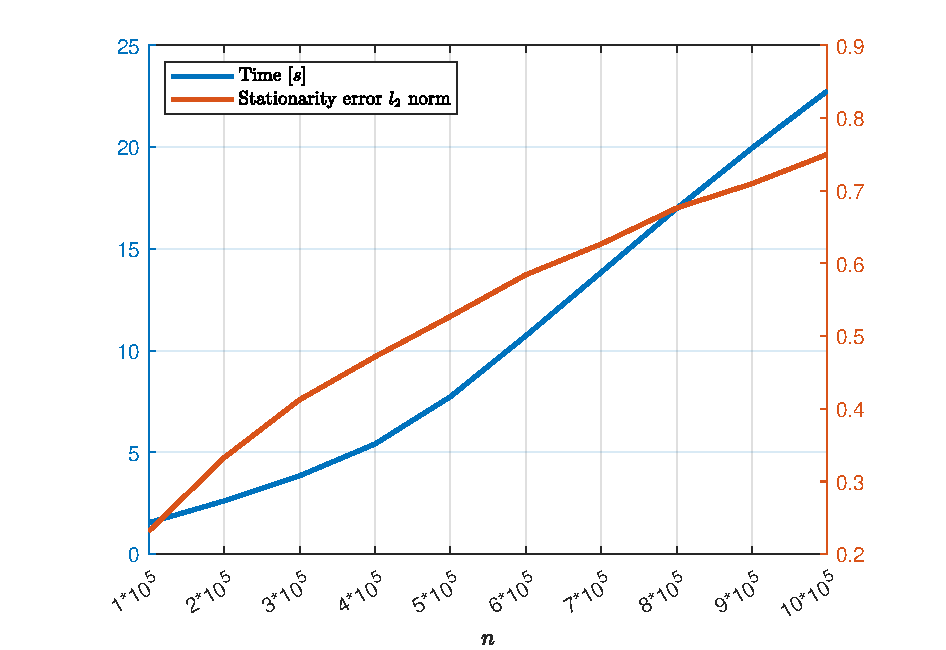
\includegraphics[scale = 0.45]{pictures/augmented_native.pdf}}
    \subfloat[2][Our GMRES implementation]{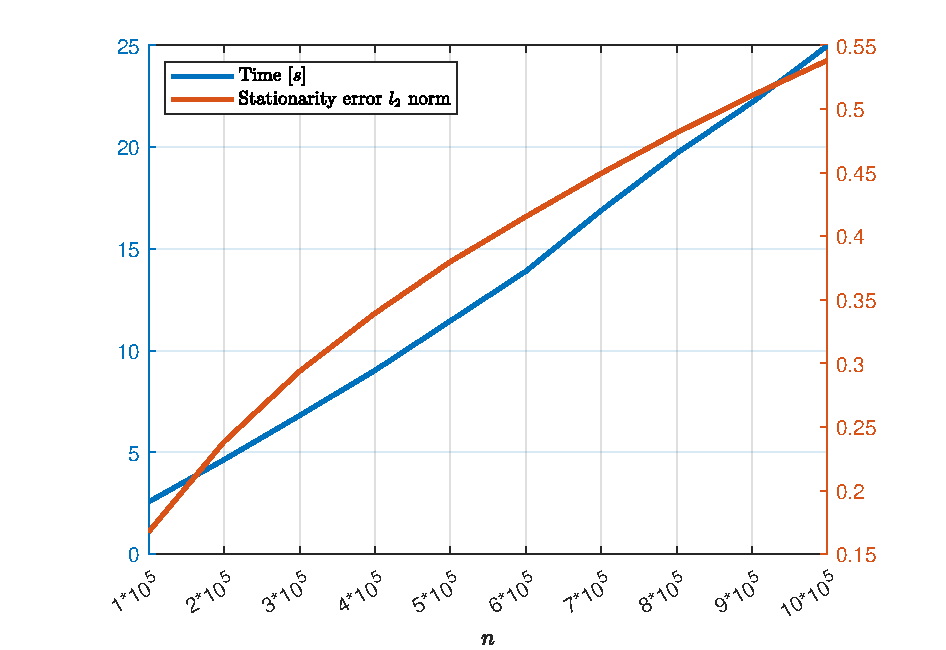
\includegraphics[scale = 0.45]{pictures/augmented_v1.pdf}}
    \caption{Time and stationarity error of the IPM algorithm using the native GMRES function implemented in MATLAB and our implementation shown for different values of \(n\).}
    \label{time_accuracy}
  \end{figure}

\noindent In \ref{time_accuracy} we can see that both computational time and accuracy of the method scale roughly linearly with the dimension of the problem. As a measure of accuracy we used the error on the stationarity condition as defined in \ref{Sec1_Eq_kkt_after}, in particular:
\[ \| Qx + c - \hat{A}^T \hat{\lambda} \| _ 2\]

\noindent A very important note is the fact that using an iterative linear system solver is \textbf{the only way to perform IPM at large scale}. We tried to solve the linear systems involved in the IPM iterations using the \textit{Backslash operator} in MATLAB (which is the standard operator to solve linear systems) but this resulted in \textbf{failing the test} when the dimension of the problem approaches \(n \sim 10^5\). Not only computational times are much higher (\(\sim 1\)min for the backslash versus \(\sim 1\)sec for the GMRES when \(n \sim 10^5\) ) but the backslash operator cannot handle the dimension of the linear system returning \texttt{NaN} as results. This could be due to the conditioning of the matrices and the lack of enough RAM memory in the system.
\\
\\
\noindent The fact that we can solve such algorithm with enough accuracy only by using an iterative linear system solver is made possible because the solution of the linear systems at each iteration does not need to be much accurate itself. The GMRES algorithm in fact stops without reaching the desired tolerance most of the time, but this is not a problem for the accuracy of the final solution. Moreover, since the maximum iterations of the GMRES algorithm are fixed, bad conditioning of the matrix does not affect computational times unlike  with the backslash operator.

\begin{figure}[H]
	\centering
	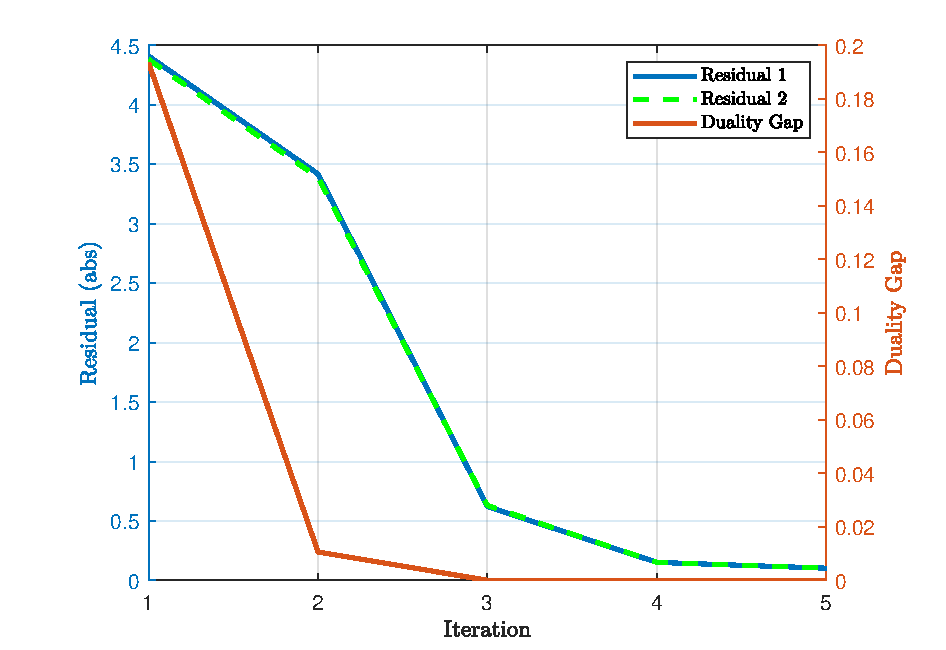
\includegraphics[scale = 0.8]{pictures/res_vs_duality.pdf}
	\caption{Residuals relative to the computation of both linear systems in each step of the IPM algorithm compared to the duality gap evolution. \(n = 10^6\), \(K = 100\)}
	\label{res_vs_duality}
\end{figure}

\noindent Since we can compute the duality gap at each step \(k\) of the IPM algorithm as:
\[
	\text{Duality Gap} = (2K + n)\mu_k\]
We can compare it to the residuals of the solutions of both linear systems in each iteration that can be easily retrieved from the GMRES algorithm as in INSERISCI REFERENCE A RESIDUO GMRES. As we can se in Figure \ref{res_vs_duality} the the magnitude of the absolute residual of both linear systems is small enough to  guarantee the convergence of the IPM algorithm in 5 iterations and the duality gap to be basically zero. 